\documentclass[11pt]{article}
\usepackage{amsmath}
\usepackage[utf8]{inputenc}
\usepackage{amsfonts,url,epsfig,breakurl}
%%% Document layout, margins
\usepackage{geometry}
\geometry{letterpaper, textwidth=6in, textheight=8.5in, marginparsep=1em}
%%% Section headings
\usepackage{sectsty}
\usepackage[normalem]{ulem}
%\setlength{\baselineskip}{40pt}

%\usepackage{hyperref}
\usepackage{todonotes}
\newcommand{\AG}[1]{\todo[inline,author=AG]{#1}}
\newcommand{\ag}[1]{\todo[size=\tiny]{ag: #1}{}}
\newcommand{\MV}[1]{\todo[inline,author=MV]{#1}}
\newcommand{\mv}[1]{\todo[size=\tiny]{mv: #1}{}}
\usepackage{verbatim}

\sectionfont{\sffamily\bfseries\upshape\large}
\subsectionfont{\sffamily\bfseries\upshape\normalsize}
\subsubsectionfont{\sffamily\mdseries\upshape\normalsize}
\makeatletter
\renewcommand\@seccntformat[1]{\csname the#1\endcsname.\quad}
\makeatother\renewcommand{\bibitem}{\vskip2pt\par\hangindent\parindent\hskip-\parindent}
\newcommand{\mme}{\mathbb{E}}

\makeatletter
\def\@maketitle{%
  \begin{center}%
  \let \footnote \thanks
    {\large \@title \par}%
    {\normalsize
      \begin{tabular}[t]{c}%
        \@author
      \end{tabular}\par}%
    {\small \@date}%
  \end{center}%
}
\makeatother


\title{\bf Bayesian analysis of tests with unknown specificity and
  sensitivity\footnote{We thank Julien Riou, Will Fithian, Sander
    Greenland, Blake McShane, Joseph Candelora, Luiz Max F.~Carvalho,
    and several reviewers for helpful comments and the National
    Science Foundation, Office of Naval Research, National Institutes
    of Health, and Schmidt Futures for financial support.  R and Stan
    code for the computations in this paper are at {\tt
      https://bob-carpenter.github.io/diagnostic-testing/}.}\vspace{.1in}}

\author{Andrew Gelman\footnote{Department of Statistics and Department
    of Political Science, Columbia University, New York.}  \ and Bob
  Carpenter\footnote{Center for Computational Mathematics, Flatiron
    Institute, New York.}  \vspace{.1in}}

\date{1 July 2020}

\begin{document}\sloppy
\maketitle

\begin{abstract}
\noindent
When testing for a rare disease, prevalence estimates can be highly
sensitive to uncertainty in the specificity and sensitivity of the
test.  Bayesian inference is a natural way to propagate these
uncertainties, with hierarchical modeling capturing variation in these
parameters across experiments.  Another concern is the people in the
sample not being representative of the general population.
Statistical adjustment cannot without strong assumptions correct for
selection bias in an opt-in sample, but multilevel regression and
poststratification can at least adjust for known differences between
the sample and the population.  We demonstrate hierarchical regression
and poststratification models with code in Stan and discuss their
application to a controversial recent study of SARS-CoV-2 antibodies in
a sample of people from the Stanford University area.  Wide posterior
intervals make it impossible to evaluate the quantitative claims of
that study regarding the number of unreported infections.  For future
studies, the methods described here should facilitate more accurate
estimates of disease prevalence from imperfect tests performed on
non-representative samples.
\end{abstract}

\section{Background}

Correction of diagnostic tests for false positives and false negatives
is a well-known probability problem.  When the base rate is low,
estimates become critically sensitive to misclassifications (Hemenway,
1997).  This issue hit the news recently (Lee, 2020), with a
study of coronavirus antibodies in a population with a low incidence
rate.

This is a problem where not fully accounting for uncertainty can make
a big difference in scientific conclusions and potential policy
recommendations.  In early April, 2020, Bendavid et al.\ (2020a)
recruited 3330 residents of Santa Clara County, California and tested
them for SARS-CoV-2 antibodies.  50 people tested positive, yielding a
raw estimate of 1.5\%.  After adjusting for differences between sample
and population in sex, ethnicity, and zip code distributions, Bendavid
et al.\ (2020a) reported an uncertainty range of 2.5\% to 4.2\%,
implying that the number of infections in the county was between 50
and 85 times the count of cases reported at the time.  Using an
estimate of the number of coronavirus deaths in the county up to that
time, they computed an implied infection fatality rate (IFR) of
0.12--0.2\%, much lower than IFRs in the range of 0.5\%--1\% that had
been estimated from areas with outbreaks of the disease.

The estimates from Bendavid et al.\ (2020a) were controversial, and it
turned out that they did not correctly account for uncertainty in the
specificity (true negative rate) of the test.  There was also concern
about the adjustment they performed for non-representativeness of
their sample.  Thus, the controversy arose from statistical adjustment
and assessment of uncertainty.  A revised preprint (Bendavid et al.,
2020b) addressed some but not all of the problems with the analysis.
It is possible that the authors of that study will prepare another
analysis for eventual publication.

In the present article we set up a Bayesian framework to clarify these
issues, specifying and fitting models using the probabilistic
programming language Stan (Carpenter et al., 2017; Stan Development
Team, 2020).  There is a long literature on Bayesian measurement-error
models (see Gustafson, 2003) and their application to diagnostic
testing (Greenland, 2009); our contribution here is to set up the
model, supply code, and consider multilevel regression and
poststratification, influence of hyperpriors, and other challenges
that arise in the problem of estimating population prevalence using
test data from a sample of people.


\section{Modeling a test with uncertain sensitivity and specificity}\label{model1}

Testing for a rare disease is a standard textbook example of
conditional probability, famous for the following counterintuitive
result. Suppose a person tests positive for a disease, based on a test
that has a 95\% accuracy rate, and further suppose that this person is
sampled at random from a population with a 1\% prevalence rate.  Then
what is the probability that he or she actually has the disease? The
usual intuition suggests that the conditional probability should be
approximately 95\%, but it is actually much lower, as can be seen from
a simple calculation of base rates, as suggested by Gigerenzer et al.\
(2007).  Imagine you test 1000 people.  With a 1\% prevalence rate, we
can expect that 10 have the disease and 990 do not.  Then, with a 95\%
accuracy rate (assuming this applies to both specificity and
sensitivity of the test), we would expect $0.95 \times 10=9.5$ true
positives and $0.05 \times 990 = 49.5$ false positives; thus, the
proportion of positive tests that are true positives (i.e., the
positive predictive value) is $9.5/(9.5+49.5) = 0.16$, a number that is
difficult to make sense of without visualizing the hypothetical
populations of true positive and false positive tests.

A related problem is to estimate the prevalence of the disease given
the rate of positive tests.  If the population prevalence is $\pi$ and
the test has a specificity of $\gamma$ and a sensitivity of $\delta$,
then the expected frequency of positive tests $p$ is
%
\begin{equation*}
  p = \pi \delta + (1- \pi)(1-\gamma)
\end{equation*}
%
Given known $\gamma$, $\delta$ and $p$, we can solve for the prevalence,
%
\begin{equation}\label{solve}
  \pi=(p + \gamma - 1)/(\delta + \gamma - 1).
\end{equation}
%
If the properties of the test are known, but $p$ is estimated from a
random sample, we can obtain a simple classical estimate by starting
with a confidence interval for $p$ and then propagating it through the
formula.  For example, Bendavid et al.\ (2020) report 50 positive
tests out of 3330, which corresponds to an estimate
$\hat{p}=50/3330=0.015$ with standard error
$\sqrt{0.015(1-0.015)/3330}=0.002$.  Supposing that their test had a
specificity of $\gamma=0.995$ and a sensitivity of $\delta=0.80$, this
yields an estimate of $(0.015 + 0.995 - 1)/(0.80 + 0.995 -1) = 0.013$
with standard error $0.002/(0.80 + 0.995 -1) = 0.003$.

Two immediate difficulties arise with the classical approach.  First,
if the observed rate $\hat{p}$ is less than $1-\gamma$, the false
positive rate of the test, then the estimate from (\ref{solve})
becomes meaninglessly negative.  Second, if there is uncertainty in
the specificity and sensitivity parameters, it becomes challenging to
propagate uncertainty through the nonlinear expression~(\ref{solve}).

We can resolve both these problems with a simple Bayesian analysis
(Gelman, 2020).  First, suppose that priors for sensitivity and
specificity have been externally supplied.  The model is then
% 
\begin{align}
\nonumber  y & \sim \mbox{binomial} (n, p) \\
 p & = (1-\gamma)(1- \pi)+ \delta\pi , \label{normals} 
\end{align}
%
along with the specified prior distribution, $p(\gamma,\delta)$.  In
this model, the parameters $\pi$, $\gamma$, and $\delta$ must be
constrained to be between 0 and 1, and $\pi$ must be given a prior
distribution too.  A natural starting point would be
$\pi\sim \mbox{uniform}(0,1)$.  In this case, previously existing
knowledge of the population prevalence was weak enough that a reasonable prior
on $\pi$ should not have much impact on the
posterior.  The three parameters $\pi$, $\gamma$, and $\delta$, are
not jointly identified from only the number of positive test cases,
hence the need for an informative prior on $\gamma$ and $\delta$. This
can be seen as a generalization of the usual approach of assuming that
these parameters are known exactly.

In the example of Bendavid (2020a), prior information on specificity
and sensitivity was given in the form of previous trials, specifically
$y_{\gamma}$ negative results in $n_{\gamma}$ tests of known negative
subjects and $y_{\delta}$ positive results from $n_{\delta}$ tests of
known positive subjects.  This yields the model,
%
\begin{align*}
   y & \sim \mbox{Binomial} (n, p)\\
  p & = (1-\gamma)(1- \pi)+ \delta\pi\\
   y_{\gamma} & \sim \mbox{Binomial} (n_{\gamma}, \gamma)\\
   y_{\delta} & \sim \mbox{Binomial} (n_{\delta}, \delta).
\end{align*}
%
We use $\mbox{uniform}(0,1)$ priors on prevalence $\pi$, specificity
$\gamma$, and sensitivity $\delta$, with the understanding that they
represent placeholders and could be augmented to include additional
information.  Stan code is in Appendix~\ref{stan2}.

We fit the model using the data reported in Bendavid et al.\ (2020a):
%
\begin{equation*}
y/n=50/3330,\qquad  y_{\gamma}/n_{\gamma}=399/401, \qquad y_{\delta}/n_{\delta} =103/122.
\end{equation*}
%
This results in high posterior uncertainty for the prevalence, $\pi$.   
%
\begin{figure}
  \centerline{ 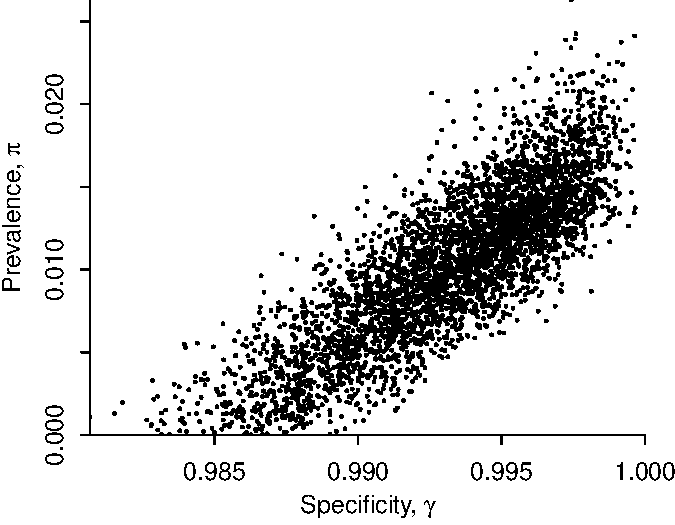
\includegraphics[width=.45\textwidth]{img/scatter.pdf}
    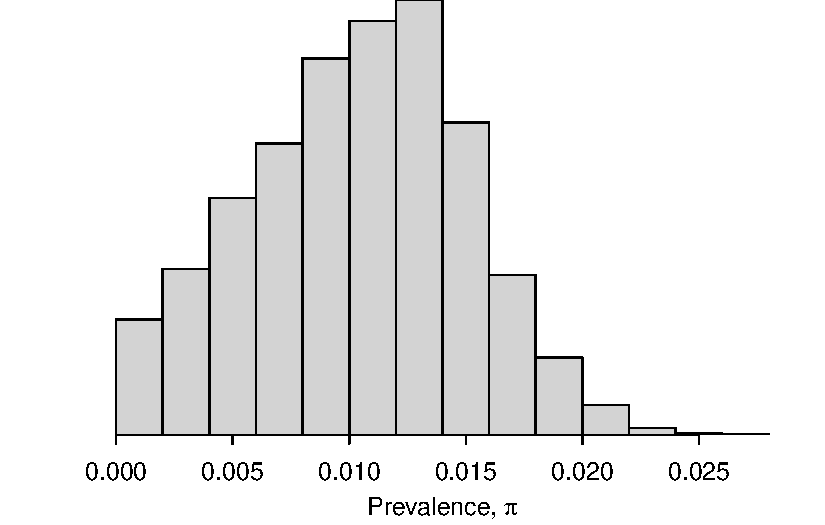
\includegraphics[width=.55\textwidth]{img/hist.pdf}}
  \caption{\em Summary of inference from model with unknown
    specificity, sensitivity, and prevalence, based on data from
    Bendavid et al.\ (2020a): (a) scatterplot of posterior simulations
    of prevalence, $\pi$, and specificity, $\gamma$; (b) histogram of
    posterior simulations of $\gamma$.  This model assumes the testing
    sites are identical and thus pools all data.}
\label{posterior1}
\end{figure}
%
Figure \ref{posterior1}a shows the joint posterior simulations for
$\pi$ and $\gamma$: uncertainty in the
population prevalence is in large part driven by uncertainty in the
specificity.  Figure \ref{posterior1}b shows the posterior
distribution for $\pi$, which reveals that the data and model are
consistent with prevalences as low as 0\% and as high as 2\%.

The asymmetric posterior distribution with its hard bound at zero
suggests that the usual central 95\% interval will not be a good
inferential summary.  Instead we the use the shortest posterior
interval%
% 
\footnote{The shortest posterior interval is equivalent to the highest
  posterior density interval for unimodal posteriors as we have here.}
%
for reasons discussed in Liu, Gelman, and Zheng
(2015). The resulting 95\% interval for $\pi$ is (0, 1.8\%), which is
much different from the intervals reported by Bendavid et al.\
(2020a,b), with or without their correction for nonrepresentativeness
of the sample.  As a result, the substantive conclusion from that
earlier report has been overturned. From the given data, the
uncertainty in the specificity is large enough that the data do not
supply strong evidence of a substantial prevalence.

\section{Hierarchical model for varying testing conditions}\label{model2}

The above analysis reveals that inference about specificity is key to
precise estimation of low prevalence rates.  In the second version of
their report, Bendavid et al.\ (2020b) include data from 13
specificity studies and 3 sensitivity studies.  Sensitivity and
specificity can vary across experiments, so it is not appropriate to
simply pool the data from these separate studies; indeed, these
particular data are not consistent with constant error rates (Fithian,
2020). We allow the parameters to vary according to a hierarchical
model where, for any study $j$, the specificity $\gamma_j$ and
sensitivity $\delta_j$ are drawn from normal distributions on the
log odds (or logistic) scale,%
%
\footnote{The log odds function is defined by $\textrm{logit}(p) = \log(p / (1 - p)).$}
%
\begin{align*}
  \mbox{logit}(\gamma_j) & \sim \mbox{normal}(\mu_{\gamma}, \sigma_{\gamma})\\
 \mbox{logit}(\delta_j) & \sim \mbox{normal}(\mu_{\delta}, \sigma_{\delta}),
\end{align*}
%
with the hyperparameters $\mu$ and $\sigma$ can be estimated from the
data.  Stan code is given in Appendix \ref{stan3}.  In general it
could make sense to allow correlation between $\gamma_j$ and
$\delta_j$ (Guo, Riebler, and Rue, 2017), but the way the data are
currently available to us, specificity and sensitivity are estimated
from separate studies and so there is no information about such a
correlation.  When coding the model, we use the convention that $j=1$
corresponds to the study of interest, with other $j > 1$ representing
studies of specificity or sensitivity given known samples.  The
parameters $\gamma_1$ and $\delta_1$ represent the specificity and
sensitivity for the site performing the prevalence study (the 50/3330
positive tests of patients with unknown status).

One could also consider alternatives to the logistic transform, which
allows the unbounded normal distribution to map to the unit interval
but might not be appropriate for tests where the specificity can
actually reach the value of 1.
%
\begin{figure}
 \begin{small}
  \centerline{
    \begin{tabular}{lccccc}
      & \multicolumn{2}{l}{(a) \it Posterior inference} &&
                                                          \multicolumn{2}{l}{(b) \it Posterior inference} \\
      & \multicolumn{2}{l}{\it with weak prior} && \multicolumn{2}{l}{\it with stronger prior} \\[6pt]
     {\it Parameter} & median & (95\% interval) && median & (95\% interval) \\\hline
     Prevalence, $\pi$ &  0.016 & (0.000, 0.160)  && 0.016 & (0.001, 0.021) \\
     Specificity, $\gamma_1$ & 0.997 & (0.987, 1.000)  && 0.995 &  (0.987, 0.999) \\
     Sensitivity, $\delta_1$ & 0.797 & (0.065, 1.000) && 0.821 & (0.622, 0.959) \\ \hline
     $\mu_{\gamma}$ & 5.54 & (4.43, 6.72) && 5.234 & (4.60, 5.91) \\
     $\mu_{\delta}$ & 1.54 & (0.24, 2.89) && 1.54 & (0.90, 2.22) \\ \hline
     $\sigma_{\gamma}$ & 1.62 & (0.82, 2.61) && 0.72 & (0.26, 1.15) \\
     $\sigma_{\delta}$ &  0.87 & (0.11, 2.16) && 0.39 & (0.00, 0.73)
  \end{tabular}
}
\end{small}
\caption{\em Summary of inferences (posterior median and shortest 95\%
  posterior interval)  for the prevalence, specificity,
  and sensitivity of the Bendavid et al.\ (2020b) study, along
  with inferences for the hyperparameters characterizing the distribution of specificity
  and sensitivity on the logistic scale.  (a) For the model with weak
  priors for $\sigma_{\gamma}$ and $\sigma_{\delta}$, the posterior
  inference for the prevalence, $\pi$, is highly uncertain.  This is
  driven by uncertainty in the sensitivity, which in turn is driven
  by uncertainty in the hyperparameters for the sensitivity
  distribution. (b) Stronger priors on $\sigma_{\gamma}$ and
  $\sigma_{\delta}$ have the effect of regularizing the specificity
  and sensitivity parameters, leading to narrower intervals for $\pi$,
  the parameter of interest in this study.  The hyperparameters $\mu$
  and $\sigma$ are on the logistic scale and thus are difficult to
  interpret without transformation.}
\label{posterior2}
\end{figure}

We fit the above hierarchical model to the data from Bendavid et al.\
(2020b), assigning a uniform prior to $\pi$ and weak
$\mbox{normal}^+(0,1)$ priors to $\sigma_{\gamma},\sigma_{\delta}$
(using the notation $\mbox{normal}^+$ for the truncated normal
distribution constrained to be positive).  We often use half-normal or
half-$t$ priors for variance parameters when we want to constrain them
at the high end but allow them to be arbitrarily close to zero if the
data support such inferences (Gelman, 2006).  Setting the scale of
these half-normals to 1 makes the prior weak for this particular
application, in the following sense. A shift of 1 on the logit scale
represents a pretty big change in sensitivity or specificity.  For
example, $\mbox{logit}(0.8)=1.4$, so if 0.8 is a typical value of
sensitivity, and if $\sigma_{\delta}=1$, then we would expect
sensitivities to vary by roughly $\pm 1$ standard
deviation, or 0.4 to 2.4 on the logit scale,
which corresponds to a probability range from 0.60 to 0.92.  The
$\mbox{normal}^+(0,1)$ hyperpriors weakly pull the specificities and
sensitivities from different studies toward each other, while allowing
for a large variation if required by the data.

The resulting posterior inference is shown in Figure
\ref{posterior2}a.  The 95\% posterior interval for the prevalence is
now $(0.000, 0.160)$.  Where does that upper bound come from: how could
an underlying prevalence of 16\% be plausible, given that only 1.5\% of
the people in the sample tested positive?  The answer can be seen from
the large uncertainty in the sensitivity parameter, which in turn
comes from the possibility that $\sigma_{\delta}$ is very large.  The
trouble is that the sensitivity information in these data comes from
only three experiments, which is not enough to get a good estimate of
the underlying distribution.  This problem is discussed by Guo,
Riebler, and Rue (2017).

The only way to make progress here is to constrain the sensitivity
parameters in some way.  One possible strong assumption is to assume
that $\sigma_{\delta}$ is some small value.  This could make sense in
the current context, as we can consider it as a relaxation of the
assumption of Bendavid et al.\ (2020b) that $\sigma_{\delta} = 0$.  We
also have reason to believe that specificity will not vary much
between experiments, so we will apply a soft constraint to the
variation in specificities as well.

Instead of specifying $\sigma_{\delta}$, we give it an informative
prior distribution.  In particular, we replace the weakly informative
$\mbox{normal}^+(0, 1)$ priors on $\sigma_{\gamma},\sigma_{\delta}$
with something stronger,
$\sigma_{\gamma}, \sigma_{\delta}\sim\mbox{normal}^+(0, 0.3)$.  To get
a sense of what this means, start with the point estimate from Figure
\ref{posterior2}a of $\mu_{\delta}$, which is 1.58. If $\sigma_{\delta}$ were 0.3, then there would be a roughly 2/3 chance that the sensitivity of
in a new experiment is in the range
$\mbox{logit}^{-1}(1.58 \pm 0.3)$, which is $(0.78, 0.87)$. This seems reasonable.

Figure \ref{posterior2}b shows the results.  Our 95\% interval for
$\pi$ is now $(0.001, 0.021)$; that is, the infection rate is
estimated to be somewhere between 0.1\% and 2.1\%.

\section{Prior sensitivity analysis}

To assess the sensitivity of the above prevalence estimate to the
priors placed on $\sigma_{\gamma}$ and $\sigma_{\delta}$, we consider
the family of prior distributions,
%
\begin{align*}
  \sigma_{\gamma} & \sim \mbox{normal}^+(0, \tau_{\gamma})\\
\sigma_{\delta} & \sim  \mbox{normal}^+(0, \tau_{\delta}),
\end{align*}
%
where $\tau_{\delta} $ and $\tau_{\gamma} $ are user-specified
hyperparameters. Setting $\tau_{\delta}$ and $\tau_{\gamma}$ to zero
would force $\sigma_{\delta}$ and $\sigma_{\gamma}$ to be zero and
would enforce complete pooling, corresponding to Bendavid et al.'s
(2020b) assumption that each test site has identical specificity and
sensitivity. As the hyperparameters are increased, the scales of
variation of $\sigma_{\gamma}$ and $\sigma_{\delta}$ are allowed to
vary more, and setting $\tau_{\gamma}$ and $\tau_{\delta}$ to infinity
would typically be considered noninformative in the sense of providing
the least amount of constraint on the sensitivities and specificities.
In practice, we often use $\mbox{normal}^+(0,1)$ priors for
hierarchical scale parameters, on the default assumption that the
underlying parameters (in this case, the specificities) will probably
vary by less than 1 on the logit scale.

For this problem, however, a weak prior does not work: as shown in the
left panel of Figure \ref{posterior2}, the resulting inferences for
the sensitivities are hopelessly wide. We do not believe these tests
have specificities below 50\%, yet such a possibility is included in
the posterior distribution, and this in turn propagates to
inappropriately wide intervals for the prevalence, $\pi$.  As
explained in the previous section, that is why we assigned a stronger
prior, using hyperprior parameters $\tau_{\gamma}=\tau_{\delta}=0.2$.

\begin{figure}
  \centerline{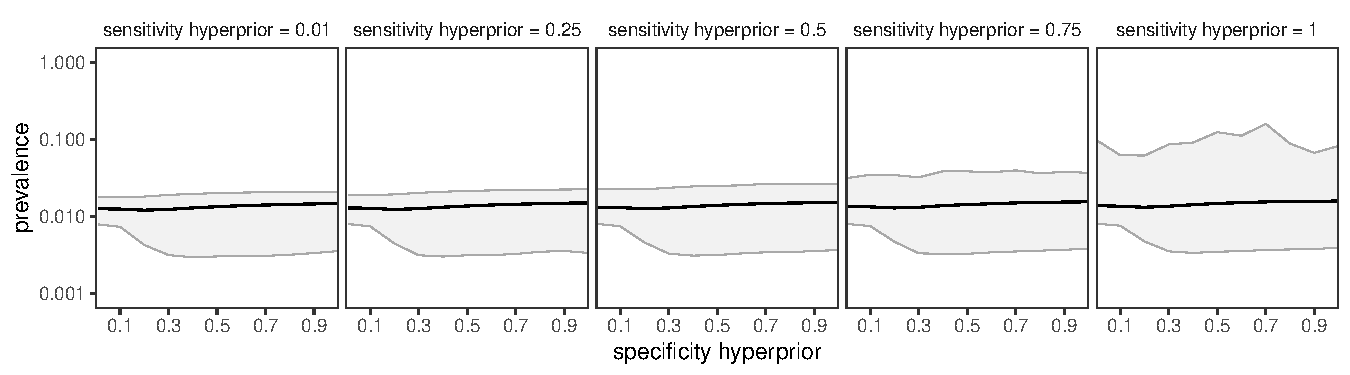
\includegraphics[width=\textwidth]{img/prior-sensitivity-2.pdf}}
  \vspace{-.15in}
\caption{\em Each panel shows a plot of the posterior median and central 90\%
  posterior interval of the prevalence, $\pi$, as a function of $\tau_{\gamma}$ and $\tau_{\delta}$, the prior scales for the specificity  and sensitivity
  hyperparameters, $\sigma_{\gamma}$ and $\sigma_{\delta}$.
  The posterior median of prevalence is not sensitive to $\tau_{\gamma}$ and $\tau_{\delta}$, but the endpoints of the 90\% interval show some sensitivity.  It is possible to use a weak hyperprior on the scale of the specificity distribution,  $\sigma_{\gamma}$:  this makes sense given that there are 13 prior specificity studies in the data.  For the scale of the sensitivity distribution,  $\sigma_{\delta}$, it is necessary to use a prior scale of 0.5 or less to effectively rule out the possibility of extremely high prevalence  corresponding to an unrealistic sensitivity parameter $\gamma$.  The noise in the rightmost graph represents Monte Carlo error that is a consequence of the weakly specified model.}\label{prior-sensitivity.fig}
\end{figure}
%
Figure~\ref{prior-sensitivity.fig} shows how these hyperprior
parameters $\tau_{\gamma}$ and $\tau_{\delta}$ affect inferences for
the prevalence, $\pi$.  The posterior median of $\pi$ is not sensitive
to the scales $\tau_{\gamma}$ and $\tau_{\delta}$ of the hyperpriors,
but the uncertainty in that estimate, as indicated by the central
posterior 90\% intervals, is influenced by these settings.  In
particular, in the graphs on the right, when the sensitivity
hyperprior parameter $\tau_{\delta}$ is given a high value, the upper
end of the interval is barely constrained.  The lower end of the
interval is fairly stable, as long as the specificity hyperprior
parameter $\tau_{\gamma}$ is not given an artificially low value. Here
we are using central rather than shortest posterior intervals because
we are displaying inference on the log scale and so there is no
boundary.

When $\tau_{\gamma}$ and $\tau_{\delta}$ are too low, the variation in
specificity and sensitivity are constrained to be nearly zero, all
values are pooled, and uncertainty is artificially deflated. As the
hyperprior parameters are increased, the uncertainty in prevalence
increases. This gets out of hand when the hyperprior for sensitivity
is increased, because there are only three data points to inform the
distribution it controls. This is an example of the general principle
that wide hyperpriors on hierarchical scale parameters can pull most
of the probability mass into areas of wide variation and dominate the
data, leading to inflated uncertainty.  Around the middle of these
ranges, the posterior intervals are not as sensitive to variation in
the hyperpriors. We would consider values
$\tau_{\gamma}=\tau_{\delta}=0.5$ to be weakly informative for this
example, in that they are roughly consistent with inter-site variation
in specificity in the range 73\% to 99.3\% and of specificity in the
range 88\% to 99.75\%.

In addition we need priors on $\mu_{\gamma}$ and $\mu_{\delta}$.  In
this particular example, once we have constrained the variation in the
specificities and sensitivities, enough data are available to estimate
these population means with uniform priors on these parameters, but in
general it is best to use prior information to at least roughly
constrain them.  For this example, we assign independent
$\mbox{normal}(4,2)$ priors, a distribution that puts 2/3 of its mass
in the range $4\pm 2$, which, after undoing the logistic
transformation, corresponds to $(0.881, 0.997)$ on the probability
scale, which seem like a suitably broad range for the mean of the
population distribution of specificity and sensitivity of these tests.

The complexity of this sensitivity analysis might seem intimidating:
if Bayesian inference is this difficult and this dependent on priors,
maybe it is not a good idea?

We would argue that the problem is not as difficult as it might look.
The steps taken in Sections \ref{model1} and \ref{model2} show the
basic workflow: We start with a simple model, then add hierarchical
structure.  For the hierarchical model we started with weak priors on
the hyperparameters and examined the inferences, which made us realize
that we had prior information (that specificities and sensitivities of
the tests should not be so variable), which we then incorporated into
the next iteration of the model.  Performing the sensitivity analysis
was fine---it helped us understand the inferences better---but it was
not necessary for us to get reasonable inferences.

Conversely, non-Bayesian analyses would not be immune from this
sensitivity to model choices, as is illustrated by the mistakes made
by Bendavid et al.\ (2020b) to treat specificity and sensitivity as
not varying at all, to set $\sigma_{\gamma}=\sigma_{\delta}=0$ in our
notation.  An alternative could be to use the calibration studies to
get point estimates of $\sigma_{\gamma}$ and $\sigma_{\delta}$, but
then there would still be the problem of accounting for uncertainty in
these estimates, which would return the researchers to the need for
some sort of external constraint or bound on the distribution of the
sensitivity parameters $\delta_j$, given that only three calibration
studies are available here to estimate these.  This in turn suggests
the need for more data or modeling of the factors that influence the
test's specificity and sensitivity.  In short, the analysis shown in
Figure \ref{prior-sensitivity.fig} formalizes a dependence on prior
information that would arise, explicitly or implicitly, in any
reasonable analysis of these data.

\section{Extensions of the model}

\subsection{Multilevel regression and poststratification (MRP) to adjust for differences between sample and population}\label{mrp}

Bendavid et al.\ (2020a,b) compared demographics on 3330 people they
tested, and they found differences in the distributions of sex, age,
ethnicity, and zip code of residence compared to the general
population of Santa Clara County. It would be impossible to
poststratify the raw data on 2 sexes, 4 ethnicity categories, 4 age
categories, and 58 zip codes, as the resulting 1856 cells would
greatly outnumber the positive tests in the data.  They obtained
population estimates by adjusting for sex $\times$ ethnicity $\times$
zip code, but their analysis is questionable, first because they did
not adjust for age, and second because of noisy weights arising from
the variables they did adjust for.  To obtain stable estimates while
adjusting for all these variables, we would recommend applying a
multilevel model to the exposure probability, thus replacing the
constant $\pi$ in the above models with something like the following logistic
regression.%
%
\footnote{$x[i]$ and $x_i$ are used interchangeably to improve readability.}
%
\begin{equation}\label{mrp.model}
\pi_i = \mbox{logit}^{-1}(\beta_1 + \beta_2 \cdot \textit{male}_i + \beta_3 \cdot x^{\textrm{zip}}_{\textit{zip}[i]} + \alpha^{\textrm{eth}}_{\textit{eth}[i]} + \alpha^{\textrm{age}}_{\textit{age}[i]} + \alpha^{\textrm{zip}}_{\textit{zip}[i]}),
\end{equation}
%
where {\it male} is a variable that takes on the value 0 for women and
1 for men; $x^{\rm zip}$ is a relevant predictor at the zip code
level; $\textit{eth}[i]$, $\textit{age}[i]$, and $\textit{zip}[i]$ are
index variables for survey respondent $i$; the $\beta$ parameters are logistic
regression coefficients; and the $\alpha$ parameters are vectors of varying
intercepts.  These varying intercepts have hierarchical priors
%
\begin{align*}
  \alpha^{\textit{name}} &\sim \mbox{normal}(0, \sigma^{\textit{name}}), \ \textrm{for} \ \textit{name} \in \{ \textrm{eth, age, zip} \}.
\end{align*}
%

In the regression model (\ref{mrp.model}), it is important to include
the predictor $x^{\textrm{zip}}$, which in this example might be
percent Latino or average income in the zip code.  Otherwise, with so
many zip codes, the multilevel model will just partially pool most of
the zip code adjustments to zero, and not much will be gained from the
geographic poststratification.  The importance of geographic
predictors is well known in the MRP literature; see, for example,
(Caughey and Warshaw 2019).

In addition, priors are needed for
$\sigma^{\textrm{eth}}, \sigma^{\textrm{age}}, \sigma^{\textrm{zip}}$,
and $\beta$, along with the hierarchical specificity and sensitivity
parameters from the earlier model.  
For these hyperparameters, we assign $\mbox{normal}^+(0, 0.5)$ priors for
$\sigma^{\textrm{eth}}$, $\sigma^{\textrm{age}}$, and
$\sigma^{\textrm{zip}}$.  These priors allow the prevalence to vary
moderately by these poststratification factors.

We use a unit logistic prior for the centered
intercept
$\beta_1 + \beta_2 \cdot \overline{\it male} + \beta_3 \cdot \overline{x}^{\rm zip}$
(corresponding to a $\mbox{uniform}(0,1)$ prior distribution for the probability that an average person in the
sample has the antibody), a $\mbox{normal}(0,0.5)$ prior for
$\beta_2$, and a $\mbox{normal}(0, 0.5/s_{\rm zip})$ for $\beta_3$, where $s_{\rm zip}$ is the standard deviation of $x_{\rm zip}$ in the data.

The point of the scaling of $\beta_2$ and $\beta_3$ is to give some prior regularization on the contribution of each predictor in the data.  Regarding the prior on the intercept:
Stan allows direct assignment of distributions to
  transformed parameters; in this particular case, the transform is
  affine and thus does not require a Jacobian adjustment.  By assigning prior distributions to the centered intercept and two other regression coefficients, we have implicitly assigned a prior distribution to the three parameters, $(\beta_1,\beta_2,\beta_3)$.

We code the model in Stan; see Appendix \ref{stan4}.  
 Unfortunately
the raw data from Bendavid et al.\ are not currently available, so we
fit the model to simulated data to check the stability of the
computation.

The above model is a start; it could be improved by including
interactions, following the general ideas of Ghitza and Gelman (2013).
In any case, once this model has been fit, it can be used to make
inferences for disease prevalence for all cells in the population. As
discussed by Johnson (2020), these cell estimates can then be summed,
weighting by known population totals (in this case, the number of
people in each sex $\times$ ethnicity $\times$ age $\times$ zip code
category in the population) to get inferences for the prevalence in
the county,
%
\begin{equation*}
  p^{\textrm{avg}}
  = \frac{\small\textstyle \sum_j N_j\pi_j}
         {\small\textstyle \sum_j N_j},
\end{equation*}
%
where $N_j$ is the
number of people in cell $j$ in the general population, and $\pi_j$ is
the prevalence in cell $j$ as computed from the logistic model.  We
perform this summation in the generated quantities block of the Stan
model in Appendix \ref{stan4}.

\subsection{Variation across location and over time}\label{muiltiple}

The aforementioned Santa Clara County study is just one of many recent
SARS-CoV-2 antibody surveys.  Other early studies were conducted in
Boston, New York, Los Angeles, and Miami, and in various places
outside the United States, and we can expect many more in the future.
If the raw data from these studies were combined, it should be
possible to estimate the underlying prevalences from all these studies
using a hierarchical model, allowing specificity, sensitivity, and
prevalence to vary by location, and adjusting for non-sampling error
where possible.  Such an analysis is performed by Levesque and Maybury
(2020) using detailed information on the different tests used in
different studies.

We will also be seeing more studies of changing infection rates over
time.  Stringhini et al.\ (2020) perform such an analysis of weekly
surveys in Geneva, Switzerland, accounting for specificity and
sensitivity and poststratifying by sex and age.

\subsection{Including additional diagnostic data}

We have so far assumed that test results are binary, but additional
information can be gained from continuous measurements that make use
of partial information when data are near detection limits (Gelman,
Chew, and Shnaidman, 2004; Bouman, Bonhoeffer, and Regoes, 2020).
Further progress can be made by performing different sorts of tests on
study participants or retesting observed positive results.

Another promising direction is to include additional information on
people in the study, for example from self-reported symptoms.  Some
such data are reported in Bendavid et al.\ (2020b), although not at
the individual level. With individual-level symptom and test data, a
model with multiple outcomes could yield substantial gains in
efficiency compared to the existing analysis using only a single
positive/negative test result on each participant.

A third direction would be to acquire test results from sites testing
both known positive and known negative cases.  With such tests,
bivariate priors for sensitivity and specificity could be formulated
as suggested by Guo, Riebler, and Rue (2017).  Simple multivariate
normal priors are possible, but the situation is complicated because,
in general, sensitivity is negatively correlated with specificity in
diagnostic tests, but above or below average testing quality at the
sites will provide positive correlation.  Thus it may be better to
formulate priors in terms of bias (trading sensitivity for
specificity) and accuracy instead of directly in terms of sensitivity
and specificity.


\section{Non-Bayesian approaches}\label{nonbayes}

As with any statistical analysis, alternative approaches are possible
that would use the same information and give similar results.

In Section \ref{model1}, it was necessary to account for uncertainty
in all three parameters, while respecting the constraint that all
three probabilities had to be between 0 and 1.  We assume that both
these aspects of the model could be incorporated into a non-Bayesian
approach by working out the region in the space of
$(\pi,\gamma,\delta)$ that is consistent with the data and then
constructing a family of tests which could be inverted to create
confidence regions.

This could be expanded into a multilevel model as in Section
\ref{model2} by considering the specificities and sensitivities of the
different experiments as missing data and averaging over their
distribution, but still applying non-Bayesian inference to the
resulting hyperparameters.  The wide uncertainty intervals from the
analysis in Section \ref{model2} suggest that some constraints or
regularization or additional information on the hyperparameters would
be necessary to get stable inferences here, no matter what statistical
approach is used.

Fithian (2020) performs a non-Bayesian analysis of the data from
Bendavid et al.\ (2020b), coming to the same basic conclusion that we
do, demonstrating that the calibration data are incompatible with a
model of constant specificity and that, once the specificity is
allowed to vary, the observed rate of positive tests in the Santa
Clara study does not allow rejection of the null hypothesis of zero
infection rate.  Had it been possible to reject zero, this would not
be the end of the story: at that point one could invert a family of
tests to obtain a confidence region, as noted above.

Finally, some rough equivalent to the poststratification adjustment in
Section \ref{mrp} could be performed using a non-Bayesian weighting
approach, using some smoothing to avoid the noisiness of raw
poststratification weights.  Similarly, non-Bayesian methods could be
used to fit regressions allowing prevalence to vary over location and
time.


\section{Discussion}

\subsection{Limitations of the statistical analysis}

Epidemiology in general, and disease testing in particular, feature
latent parameters with high levels of uncertainty, difficulty in
measurement, and uncertainty about the measurement process as well.
This is the sort of setting where it makes sense to combine
information from multiple studies, using Bayesian inference and
hierarchical models, and where inferences can be sensitive to
assumptions.

The biggest assumptions in this analysis are, first, that the
historical specificity and sensitivity data are relevant to the
current experiment; and, second, that the people in the study are a
representative sample of the general population.  We addressed the
first concern with a hierarchical model of varying sensitivities and
specificities, and we addressed the second concern with multilevel
regression and poststratification on demographics and geography.  But
this modeling can take us only so far.  If there is hope or concern
that the current experiment has unusual measurement properties, or
that the sample is unrepresentative in ways not accounted for in the
regression, then more information or assumptions need to be included
in the model, as described by Campbell et al.\ (2020).

The other issue is that there are choices of models, and tuning
parameters within each model.  Sensitivity to the model is apparent in
Bayesian inference, but it would arise with any other statistical
method as well.  For example, Bendavid et al.\ (2020a) used an
(incorrectly applied) delta method to propagate uncertainty, but this
is problematic when sample size is low and probabilities are near 0 or
1.  Bendavid et al.\ (2020b) completely pooled their specificity and
sensitivity experiments, which is equivalent to setting
$\sigma_{\gamma}$ and $\sigma_{\delta}$ to zero.  And their weighting
adjustment has many arbitrary choices.  We note these not to single
out these particular authors but rather to emphasize that, at least
for this problem, all statistical inferences involve user-defined
settings.

For the models in the present article, the most important user choices
are: (a) what data to include in the analysis, (b) prior distributions
for the hyperparameters, and (c) the structure and interactions to
include in the MRP model.  For these reasons, it would be difficult to
set up the model as a plug-and-play system where users can just enter
their data, push a button, and get inferences.  Some active
participation in the modeling process is required, which makes sense
given the sparseness of the data.  When studying populations with
higher prevalences and with data that are closer to random samples,
more automatic approaches might be possible.

\subsection{Santa Clara study}

Section \ref{model2} shows our inferences given the summary data in
Bendavid et al.\ (2020b).  The inference depends strongly on the
priors on the distributions of sensitivity and specificity, but that
is unavoidable: the only way to avoid this influence of the prior
would be to sweep it under the rug, for example by just assuming a
zero variation in the test parameters.

What about the claims regarding the rate of coronavirus exposure and
implications for the infection fatality rate?  It is hard to say from
this one study: the numbers in the data are consistent with zero
infection rate and a wide variation in specificity and sensitivity
across tests, and the numbers are also consistent with the claims made
in Bendavid et al.\ (2020a,b). That does not mean anyone thinks the
true infection rate is zero.  It just means that more data,
assumptions, and subject-matter knowledge are required. That is to be
expected---people usually make lots of assumptions in analyzing this
sort of laboratory assay. It is common practice to use the
manufacturer's numbers on specificity, sensitivity, detection limit,
and so forth, and not worry about that level of variation. Only when
estimating a very low underlying rate do the statistical challenges
become so severe. This is an example of the general phenomenon in
statistics that the severity of identification problems can depend on
the data.

For now, we do not think the data support the claim that the number of
infections in Santa Clara County was between 50 and 85 times the count
of cases reported at the time, or the implied interval for the IFR of
0.12--0.2\%.  These numbers are consistent with the data, but the data
are also consistent with a near-zero infection rate in the county.
The data of Bendavid et al.\ (2020a,b) do not provide strong evidence
about the number of people infected or the infection fatality ratio;
the number of positive tests in the data is just too small, given
uncertainty in the specificity of the test.

The analyses in this article suggest that future studies should be
conducted with full awareness of the challenges of measuring
specificity and sensitivity, that relevant variables be collected on
study participants to facilitate inference for the general population,
and that (de-identified) data be made accessible to external
researchers.


\section*{References}

\noindent

\bibitem Bendavid, E., Mulaney, B., Sood, N., Shah, S., Ling, E.,
  Bromley-Dulfano, R., Lai, C., Weissberg, Z., Saavedra-Walker, R.,
  Tedrow, J., Tversky, D., Bogan, A., Kupiec, T., Eichner, D., Gupta,
  R., Ioannidis, J., and Bhattacharya, J. (2020a).  COVID-19 antibody
  seroprevalence in Santa Clara County, California, version 1. {\small
    \url{https://www.medrxiv.org/content/10.1101/2020.04.14.20062463v1.full.pdf}}

\bibitem Bendavid, E., Mulaney, B., Sood, N., Shah, S., Ling, E.,
  Bromley-Dulfano, R., Lai, C., Weissberg, Z., Saavedra-Walker, R.,
  Tedrow, J., Tversky, D., Bogan, A., Kupiec, T., Eichner, D., Gupta,
  R., Ioannidis, J., and Bhattacharya, J. (2020b).  COVID-19 antibody
  seroprevalence in Santa Clara County, California, version 2. {\small
    \url{https://www.medrxiv.org/content/10.1101/2020.04.14.20062463v2.full.pdf}}

\bibitem Bouman, J. A., Bonhoeffer, S., and Regoes, R. R.  (2020).
  Estimating seroprevalence with imperfect serological tests: a
  cutoff-free approach.  {\small
    \url{https://www.biorxiv.org/content/10.1101/2020.04.29.068999v2}}

\bibitem Campbell, H., de Valpine, P., Maxwell, L., de Jong, V. M. T.,
  Debray, T., Jänisch, T., and Gustafson, P. (2020).  Bayesian
  adjustment for preferential testing in estimating the COVID-19
  infection fatality rate: Theory and methods.  {\small
    \url{https://arxiv.org/abs/2005.08459}}

\bibitem Carpenter, B., Gelman, A., Hoffman, M.~D., Lee, D., Goodrich,
  B, Betancourt, M., Brubaker, M., Guo, J., Li, P., and Riddell, A.
  (2017). Stan: A probabilistic programming language. {\em Journal of
    Statistical Software} {\bf 76} (1), 1--32. {\small
    \url{https://www.jstatsoft.org/article/view/v076i01}}

\bibitem Caughey, D., and Warshaw, C. (2019).  Public opinion in
  subnational politics.  {\em Journal of Politics} {\bf 81}, 352--363.

\bibitem Fithian, W. (2020).  Statistical comment on the revision of
  Bendavid et al. {\small
    \url{https://www.stat.berkeley.edu/~wfithian/overdispersionSimple.html}}

\bibitem Gelman, A. (2006). Prior distributions for variance
  parameters in hierarchical models. {\em Bayesian Analysis} {\bf 1},
  515--533.
  
\bibitem Gelman, A. (2020).  Simple Bayesian analysis inference of
  coronavirus infection rate from the Stanford study in Santa Clara
  county. {\em Statistical Modeling, Causal Inference, and Social
    Science}, 1 May.  {\small \url{https://statmodeling.stat.columbia.edu/2020/05/01/simple-bayesian-analysis-inference-of-coronavirus-infection-rate-from-the-stanford-}} {\small \url{study-in-santa-clara-county}}
  
\bibitem Gelman, A., Chew, G., and Shnaidman, M. (2004).  Bayesian
  analysis of serial dilution assays. {\em Biometrics} {\bf 60},
  407--417.

\bibitem Ghitza, Y., and Gelman, A., (2013). Deep interactions with
  MRP: Election turnout and voting patterns among small electoral
  subgroups. {\em American Journal of Political Science} {\bf 57},
  762--776.

\bibitem Gigerenzer, G., Gaissmaier, W., Kurz-Milcke, E., Schwartz,
  L. M., and Woloshin, S.  (2007).  Helping doctors and patients make
  sense of health statistics.  {\em Psychological Science in the
    Public Interest} {\bf 8}, 53--96.

\bibitem Greenland, S. (2009).  Bayesian perspectives for
  epidemiologic research: III. Bias analysis via missing-data methods.
  {\em International Journal of Epidemiology} {\bf 38}, 1662--1673.

\bibitem Guo, J., Riebler, A., and Rue, H. (2017).  Bayesian bivariate
  meta-analysis of diagnostic test studies with interpretable priors.
  {\em Statistics in Medicine} {\bf 36}, 3039--3058.

\bibitem Gustafson, P. (2003).  {\em Measurement Error and
    Misclassification in Statistics and Epidemiology: Impacts and
    Bayesian Adjustments}.  London: CRC Press.

\bibitem Hemenway, D. (1997).  The myth of millions of annual
  self-defense gun uses: A case study of survey overestimates of rare
  events.  {\em Chance} {\bf 10} (3), 6--10.

\bibitem Johnson, D. (2020).  Estimating seroprevalence with data from
  an imperfect test on a convenience sample.  {\small
    \url{https://www.dougjohnson.in/post/estimating-seroprevalence-}} {\small \url{with-data-from-an-imperfect-test-on-a-convenience-sample/}}

\bibitem Lee, S. M. (2020).  Two antibody studies say coronavirus
  infections are more common than we think. Scientists are mad.  {\em
    BuzzFeed News}, 22 Apr.  {\small
    \url{https://www.buzzfeednews.com/article/stephaniemlee/coronavirus-antibody-test-santa-clara-los-angeles-stanford}}

\bibitem Levesque, J., and Maybury, D. W. (2020).  A note on COVID-19
  seroprevalence studies: a meta-analysis using hierarchical
  modelling.  {\small
    \url{https://www.medrxiv.org/content/10.1101/2020.05.03.20089201v1.full.pdf}}

\bibitem Liu, Y., Gelman, A., and Zheng, T. (2015).
  Simulation-efficient shortest probability intervals. {\em Statistics
    and Computing} {\bf 25}, 809--819.

\bibitem Stan Development Team (2020). {\em Stan User's Guide}. Version
  2.23. {\small \url{https://mc-stan.org/docs/2_23/stan-users-guide/index.html}}

\bibitem Stringhini, S., Wisniak, A., Piumatti, G., Azman, A. S.,
  Lauer, S. A., Baysson, H., De Ridder, D., Petrovic, D., Schrempft,
  S., Marcus, K., Yerly, S., Vernez, I. A., Keiser, O., Hurst, S.,
  Posfay-Barbe, K. M., Trono, D., Pittet, D., Getaz, L., Chappuis, F.,
  Eckerle, I., Vuilleumier, N., Meyer, B., Flahault, A., Kaiser, L.,
  and Guessous, I. (2020).  Repeated seroprevalence of anti-SARS-CoV-2
  IgG antibodies in a population-based sample.  {\small
    \url{https://www.medrxiv.org/content/10.1101/2020.05.02.20088898v1.full.pdf}}

\pagebreak
\appendix

\section{Stan programs}

\subsection{Model with binomial data on specificity and sensitivity}\label{stan2}

\vspace{-\baselineskip}
\begin{small}
  \begin{quotation}\noindent
    \verbatiminput{stan/santa-clara.stan}
  \end{quotation}
\end{small}


\subsection{Hierarchical model for specificities and sensitivities}\label{stan3}

\vspace{-\baselineskip}
\begin{small}
  \begin{quotation}\noindent
    \verbatiminput{stan/santa-clara-hierarchical.stan}
  \end{quotation}
\end{small}

\subsection{Multilevel regression and poststratification}\label{stan4}

\vspace{-\baselineskip}
\begin{small}
  \begin{quotation}\noindent
    \verbatiminput{stan/santa-clara-hierarchical-mrp.stan}
  \end{quotation}
\end{small}

\end{document}
